%%%%%%%%%%%%%%%%%%%%%%%%%%%%%%%%%%%%%%%%%%%%%%%%%%%%%%%%%%%%%%%%%%%%%%%%%%%%%%%%
%2345678901234567890123456789012345678901234567890123456789012345678901234567890
%        1         2         3         4         5         6         7         8
 
\documentclass[letterpaper, 10 pt, conference]{ieeeconf}  % Comment this line out if you need a4paper

%\documentclass[a4paper, 10pt, conference]{ieeeconf}      % Use this line for a4 paper

\IEEEoverridecommandlockouts                              % This command is only needed if 
                                                          % you want to use the \thanks command

\overrideIEEEmargins                                      % Needed to meet printer requirements.
\pdfminorversion=4
% See the \addtolength command later in the file to balance the column lengths
% on the last page of the document

% The following packages can be found on http:\\www.ctan.org
%\usepackage{graphics} % for pdf, bitmapped graphics files
%\usepackage{epsfig} % for postscript graphics files
%\usepackage{mathptmx} % assumes new font selection scheme installed
%\usepackage{times} % assumes new font selection scheme installed
%\usepackage{amsmath} % assumes amsmath package installed
%\usepackage{amssymb}  % assumes amsmath package installed

\usepackage{amssymb}
\setcounter{tocdepth}{3}
\usepackage{graphicx}
\usepackage{url}

\usepackage{amsmath} % assumes amsmath package installed
\usepackage{amssymb}  % assumes amsmath package installed
\renewcommand{\UrlFont}{\small\tt}
\usepackage{graphicx}
\usepackage{listings}
\usepackage{courier}
 \lstset{
         %basicstyle=\footnotesize\ttfamily, % Standardschrift
         basicstyle=\scriptsize\ttfamily, % Standardschrift
         %numbers=left,               % Ort der Zeilennummern
         numberstyle=\tiny,          % Stil der Zeilennummern
         %stepnumber=2,               % Abstand zwischen den Zeilennummern
         numbersep=5pt,              % Abstand der Nummern zum Text
         tabsize=1,                  % Groesse von Tabs
         extendedchars=true,         %
         breaklines=true,            % Zeilen werden Umgebrochen
         %keywordstyle=\color{red},            frame=b,
 %        keywordstyle=[1]\textbf,    % Stil der Keywords
 %        keywordstyle=[2]\textbf,    %
 %        keywordstyle=[3]\textbf,    %
 %        keywordstyle=[4]\textbf,   \sqrt{\sqrt{}} %
         stringstyle=\color{white}\ttfamily, % Farbe der String
         showspaces=false,           % Leerzeichen anzeigen ?
         showtabs=false,             % Tabs anzeigen ?
         xleftmargin=17pt,
         framexleftmargin=17pt,
         framexrightmargin=5pt,
         framexbottommargin=4pt,
         %backgroundcolor=\color{lightgray},
         showstringspaces=false      % Leerzeichen in Strings anzeigen ?
 }
\lstloadlanguages{% Check Dokumentation for further languages ...
         %[Visual]Basic
         %Pascal
         %C
         %C++
         XML
         %HTML
         %Java
 }
 
\usepackage{caption}
\DeclareCaptionFormat{listing}{\colorbox[cmyk]{0, 0,0,0}{\parbox{\columnwidth}{\hspace{15pt}#1#2#3}}}
\captionsetup[lstlisting]{format=listing,singlelinecheck=false, margin=0pt}
 
\usepackage{color}
\usepackage[tight]{subfigure}
\usepackage{balance}
\usepackage[ruled,vlined]{algorithm2e}
\usepackage{courier}

\urldef{\mailsa}\path|{jorgemunoz, imaza, aollero}@us.es|

\title{\LARGE \bf
Combining task allocation and symbolic planning for aerial robots equipped with manipulators in assembly operations*
}

\author{Jorge Munoz-Morera, Ivan Maza and Anibal Ollero% <-this % stops a space
\thanks{*This work has been partially supported by the ARCAS Project (FP7-ICT-287617) funded by the EU FP7 and the RANCOM (P11-TIC-7066) and AEROMAIN (DPI2014-59383-C2-1-R) national projects}% <-this % stops a space
\thanks{Grupo de Rob\'{o}tica, Visi\'{o}n y Control, Universidad de Sevilla, Camino de los Descubrimientos s/n, 41092 Sevilla, Spain.
\mailsa
}%
}

\begin{document}

\maketitle
\thispagestyle{empty}
\pagestyle{empty}

\graphicspath{{./}{./figures/}}

%%%%%%%%%%%%%%%%%%%%%%%%%%%%%%%%%%%%%%%%%%%%%%%%%%%%%%%%%%%%%%%%%%%%%%%%%%%%%%%%
\begin{abstract}
This work addresses the combination of task allocation and symbolic planning in missions involving a team of aerial robots assembling a structure. Each planner has its own problem domain and search space, and the paper describes how both planners interact in a loop sharing information in order to improve the solutions. The symbolic planner estimates the cost of the sequence of actions needed in the mission execution for each assignment computed and gives feedback to the task allocation planner in the search for a better assignment. This interaction scheme has been tested with different solvers at the task allocation planner level. The paper presents simulation results that show the feasibility of the approach and the performance obtained with the different solvers.
\end{abstract}
\begin{keywords}
Aerial Robotics; Planning, Scheduling and Coordination; Robotics in Construction; Assembly
\end{keywords}

%%%%%%%%%%%%%%%%%%%%%%%%%%%%%%%%%%%%%%%%%%%%%%%%%%%%%%%%%%%%%%%%%%%%%%%%%%%%%%%%
\section{INTRODUCTION AND RELATED WORK}
	\label{sec:intro}

The work described in this paper is part of the ARCAS European Project~\footnote{http://www.arcas-project.eu} funded by the European Commission. One of the goals of this project is to build a structure by using a team of aerial robots equipped with on-board manipulators. The practical interest of this system can be found in situations where it is required to build a structure in places with difficult access by conventional means. Different scheduling and planning problems are involved in this context: assembly planning, multi-robot task allocation, symbolic planning and motion planning. There is a huge amount of related work in any of these topics independently, but the problem of combining these different planning levels has been less addressed in the literature. 

Assembly planning is the process of creating a detailed assembly plan to build a structure from separate parts by taking into account the final geometry, available resources to build that structure, fixture design, feeder and tool descriptions, etc. The assembly planning problem has been shown to be an NP-complete problem~\cite{Kavraki93}. Reference~\cite{Jimenez2011} presents a survey on assembly sequencing from a combinatorial and geometrical perspective. A system on which teams of quadrotors assemble a 2.5-D structure from simple parts can be found in~\cite{Lindsey-RSS-11}. In that work the robots were equipped with grippers and the structure was supposed to be assembled sequentially, so no manipulation planning was done after picking the parts and the assembly tasks were not parallelizable. 

This paper is focused on the combination of multi-robot task allocation and symbolic planning in the context of structure assembly. Some works use task decomposition prior to the allocation of tasks, but few combine task allocation with symbolic planning. For instance, a formal method definition for task decomposition can be found in~\cite{Shi2012}, presenting also a reputation-based task allocation model for multi-robot collaboration systems. In~\cite{Zhou2011} a dual-arm robot system for inner space-station operations is presented, using task decomposition and task allocation on the higher layer. A peer search algorithm which considers the dependencies and precedence for the allocation of given decomposed tasks in multi-robot systems can be found in~\cite{Nagarajan2014}. These works present a task allocation module which depends on the previous decomposition of the different tasks, but none of them have symbolic planning capabilities. An automated assembly system that uses a team of heterogeneous robots for the assembly of furniture is presented in~\cite{Knepper2013}. In that work, a symbolic planner determines the order of operations over the parts for the assembly. However, the allocation of tasks to robots is done at the symbolic level by using preconditions and postconditions in an object-oriented symbolic planning specification language, so the task allocation does not use any optimization heuristic. 

This paper is structured as follows. The problem solved with the combination of multi-robot task allocation and symbolic planning is formally presented in Sect.~\ref{sec:pdef}. The assembly tasks are assigned to the available aerial robots by the task allocation planner described in Sect.~\ref{sec:tap}. This planner optimizes the computed assignment by calling the symbolic planner explained in Sect.~\ref{sec:assembly_symbolic}, which estimates the cost of the sequence of actions needed in the mission execution for the given assignment and gives feedback to the task allocation planner in the search for a better assignment. Section~\ref{sec:score_calc} explains the connection between the task allocation planner and the symbolic planner. Section~\ref{sec:results} includes simulation results to compare different solver configurations. Section~\ref{sec:conclusions} closes the paper with the conclusions and future work.

\section{PROBLEM STATEMENT}
	\label{sec:pdef}

Let us consider a mission $\mathcal{M}$ consisting on the assembly of a structure composed by several parts initially located around the environment. The parts have to be assembled on specific locations by a team of $n$ aerial robots starting the mission from their home locations. Then the mission is composed by a set of assembly tasks $\mathcal{T}$. Each of the parts has a weight and a dependency list consisting on the tasks that must be done prior to its assembly. Let us define $\mathcal{L}$ as the set of stock parts locations, $\mathcal{L'}$ as the set of locations where the parts have to be assembled and $\mathcal{H}$ as the home locations of the aerial robots. The objective is to assemble all the parts on their locations minimizing the travel flight times of the vehicles and exploiting the potential parallelism that can be achieved using multiple aerial robots.
    
The implicit combinatorial problem can be expressed by the edges of a graph $G(V,E)$ considering the following notation:
    
    \begin{itemize}
    	\item $\mathcal{T} = \{t_1, t_2, ..., t_m\}$ is a set of $m$ assembly tasks.
    	\item ${P_{i}} \subseteq \mathcal{T}  $ is the set of preconditions for the $i$-th task, i.e. the subset of tasks that must have been done prior to the execution of that task.
    	\item $n$ is the number of aerial robots.
    	\item $\mathcal{L} = \{l_1, l_2, ..., l_m\}$ is the set of stock parts locations and $\mathcal{L'} = \{l'_1, l'_2, ..., l'_m\}$ is the set of final assembly locations.    
    	\item $\mathcal{H} = \{h_1, h_2, ..., h_n\}$ is the set of aerial robots home locations.
  		\item $V=\{\mathcal{L}\cup\mathcal{L'}\cup\mathcal{H}\}=\{v_1, v_2, ..., v_{2m+n}\}$ is the set of vertices of the $G$ graph.
		\item $E=\{(v_i,v_j) | v_i,v_j \in V; i<j\}$ is the edge set.  		
  		\item ${R_{k} = \{r_1, r_2, ..., r_s} \}\subseteq$ $V$ is the route for the $k$-th aerial robot, composed by a subset of $s$ vertices from $V$.
		\item Cost $c_{r_i,r_j}$ is a non-negative travel time between vertex $r_i$ and $r_j$, where $c_{r_i,r_j}=c_{r_j,r_i}$.
		\item $p = \{p_1, p_2, ..., p_n\}$ is a vector with the maximum payloads of the aerial robots.
		\item $w = \{w_1, w_2, ..., w_m\}$ is a vector containing the weights of the parts.
		\item $q = \{q_1, q_2, ..., q_m\}$ is a vector containing the times on which the parts are finally assembled.
	\end{itemize}
	
The problem consists in determining a set $\mathcal{R}$ of routes with minimal cost and a vector $q$ of minimal task assembly times, with each route starting at the home locations of the vehicles, such that every vertex in $\mathcal{L}$ is visited at least by one vehicle and followed by its subsequent vertex in $\mathcal{L'}$, without exceeding the payload of each vehicle and respecting the preconditions for each of the parts. The same location can be visited by several aerial robots because some parts must be transported cooperatively by more than one aerial robot if they are too heavy. The problem described is similar to the well-known Vehicle Routing Problem (VRP)~\cite{Dantzig_Ramser_VRP}.	
	For the $k$-th aerial robot, the cost of a route is given by 

 \begin{equation}
 	{C(R_{k}) = \sum_{i=1}^{s-1} c_{r_i,r_{i+1}}} \, ,
 	\label{eq:route_cost}
 \end{equation}	

\noindent where ${r_1 \in \mathcal{H}}$, ${r_i \in V}$ and ${r_j \in}$ $\mathcal{L}$ ${\implies r_{j+1} \in}$ $\mathcal{L'}$. Considering that up to two aerial robots can cooperatively transport a single heavy part, this route ${R_{k}}$ is feasible if ${(p_k \geq w_j) \lor (\exists R_{z} | r_j \in R_{z} \land (p_k+p_z) \geq w_j)}$, i.e. the weight of each part does not exceed the maximum payload of the aerial robot transporting it or there is another available aerial robots so that both can transport it cooperatively. For each part $w_j$ in this route it must be met in addition that $\forall t_{s} \in P_{j}: q_{s}<q_{j}$, i.e. all the parts from its set of preconditions must have been assembled before that part.
	
The goal is to minimize the total travel time $\sum_{i=1}^{n} C(R_{i})$ of the feasible routes executing all the assembly tasks of the mission and balance the workload of the different aerial robots.

\section{SYMBOLIC PLANNER}
	\label{sec:assembly_symbolic}

The input for the planning engine is the 3D CAD model of the structure that has to be built. The assembly plan is computed by an assembly planner by using the well-known \emph{assembly-by-disassembly} technique~\cite{Jimenez2011}, consisting on finding a plan to disassemble the whole structure and reversing the order of its operations to get the final assembly plan. The assembly planner is out of the scope of this paper, but some details can be found in~\cite{munoz_icuas15}. In the assembly plan, each assembly task represents the assembly of one specific part of the structure and contains the preconditions that must be met prior to its execution, namely the assembly tasks that must be done before the assembly of that specific part. The only requirement to execute an assembly task from the plan is to have its preconditions met. That feature makes the computed assembly plan totally independent from the number of vehicles available for its execution. On the other hand, all the assembly tasks that have their preconditions met at any given time could be executed in parallel if there are enough robots available, decreasing the assembly time. Finally, those assembly tasks that must be executed cooperatively require synchronization among the involved aerial robots.

The JSHOP2 symbolic planner~\cite{Nau03shop2} has been chosen to deal with all these aspects of the assembly operations and to produce low-level plans for each aerial robot. JSHOP2 is a domain-independent planning system based on Hierarchical Task Networks (HTN) that decomposes tasks into smaller subtasks and so on, until obtaining low-level subtasks that can not be further decomposed. This type of symbolic planner has been chosen due to his successful application in the Robotics area in the last years. To know how to decompose tasks, JSHOP2 needs the definition of a planning domain specified by using a format very similar to a Planning Domain Definition Language (PDDL) description. In the domain, high-level task methods must be defined to represent the tasks to decompose. The task methods contain a number of preconditions in the form of logical expressions. In a given state, if the preconditions are met then the effect of applying the high-level task method over a task is its decomposition on smaller subtasks methods,  whose preconditions must also be met in order to be decomposed again until obtaining the lowest-level subtasks. Then, a task is said to be feasible if the preconditions of its task method and the preconditions of all its lower-level subtasks methods are all true, in which case the task is decomposed.

\subsection{Symbolic Domain}
\label{sec:jshop2_domain}

In JSHOP2 the current state of the world is composed by a set of logical predicates that define the entities and states that take part in the planning process. Taking into account the problem definition in Sect.~\ref{sec:pdef}, the following elements should be present in the symbolic domain:

    \begin{itemize}
    	\item The assembly parts and their preconditions lists.
        \item The initial and final poses of the parts in the structure.
        \item The aerial robots and their home locations.
        \item The number of parts that remain unassembled.
        \item An assignment of assembly tasks (parts) to aerial robots.
	\end{itemize}

The designed domain has one high-level task method defined to try to decompose all the assembly tasks assigned to the aerial robots and to find an optimal scheduling for the subtasks. The defined high-level task method is recursive, and on each call it selects one part from the set of parts that have all the preconditions met. Once selected, the aerial robots that are assigned to execute that assembly task are checked and the assembly task is tried to be decomposed into an ordered set of smaller subtasks that conform the low-level plans for the involved aerial robots. This process is repeated until all the parts are assembled. Listing~\ref{jshop2_domain} shows a simplified high-level task method definition that recursively picks a part that is assigned to only one aerial robot.

\lstinputlisting[label=jshop2_domain,caption={JSHOP2 simplified high-level task method for the assembly domain. The planner checks if there are remaining parts to be assembled and selects one among the set of parts that have all the preconditions met. This is done by retrieving the dependency list of a part and checking if all the parts that are present in that dependency list have been assembled. If that is the case, then the aerial robot assigned to assemble that part is retrieved and the assembly task is tried to be decomposed by calling a lower-level method. The case of parts that need to be transported by two aerial robots cooperatively is not shown here.}]{listings/jshop2_domain.txt}

The subtasks on which an assembly task is decomposed include operations such as take-off, move to specific locations, pick and place parts, or synchronize the aerial robots when the assembly task is cooperative. During the assembly task decomposition, the symbolic planner makes a cost estimation for each of the subtasks. This cost estimation represents the time needed to execute the subtask, that is, its duration. In addition to the duration, the planner computes the start time of the given subtasks. Having an estimation of the start time and duration of each of the subtasks makes possible to have the low-level plans of each of the involved aerial robots well ordered in time. A decomposition example of a cooperative assembly task is illustrated in Fig.~\ref{fig:timelines}.

	\begin{figure}
   		\centering
   		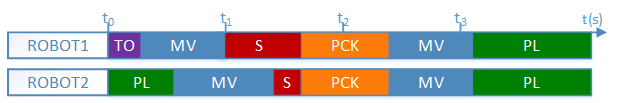
\includegraphics[width=0.99\columnwidth]{timeline.png}
   		\caption[Decomposition example of a cooperative assembly task.]{Decomposition example of a cooperative assembly task computed by the symbolic planner. The assembly task consists on assembling a part on a specific assembly location. Due to its weight, the part was assigned to be assembled by using two aerial robots. The computed timelines for the two robots are shown. Each of the boxes in the timeline represent a subtask on which the original assembly task has been decomposed by the symbolic planner. The first robot, which was initially idle before $t_0$, takes-off (TO) and move (MV) to the part location. After that, a synchronization subtask (S) is needed to wait for the second robot (which is initially finishing another assembly task) to be in its part location pose. When the second robot arrives, it synchronizes with the first. After that, the two aerial robots pick (PCK), move and place (PL) the part cooperatively in the corresponding assembly location. The subtasks start time and duration estimations are computed by the symbolic planner.}
   		\label{fig:timelines}
	\end{figure}

\section{TASK ALLOCATION PLANNER}
\label{sec:tap}

The planner chosen to solve the assignment problem presented in Sect.~\ref{sec:pdef} was OptaPlanner~\cite{optaplanner}, an open source, multi-platform planning engine written in Java. It is capable of generating near-optimal plans by applying optimization heuristics and meta-heuristics combined with score calculation. It has been chosen because the solver's algorithm is highly configurable: it is possible to use different heuristics and meta-heuristics algorithms applied in sequence, so that the user can select the most suitable for the problem in question. The optimization is based on a score calculation that is computed after all the planning entities have been assigned. This score determines the suitability of the last computed solution: if after searching for a new solution the new score is worse than the score calculated in the previous solution, then the last solution is discarded and the process continues trying to generate a solution with a better score.

\subsection{Solver Phases}
\label{sec:solver_phases}

As it was mentioned before, the OptaPlanner solver can use multiple optimization algorithms in sequence. Each of the optimization algorithms used is called a solver phase. During the execution of the solver there is never more than one solver phase executing at the same time, so a solver phase only starts when the previous phase has finished. There are three types of solver phases that can be used in the OptaPlanner solver: Construction Heuristics (CH), Metaheuristics (MH) and Exhaustive Search (ES). 

The CH solver phase builds an initial solution in a short time. The solution computed is not always feasible, but it tries to find it fast so that the following solver phases can finish the search of a feasible one by starting from that initial solution. There are different algorithms that can be used as CH. One common characteristic of them is that when a CH assigns a planning entity, that assignment remains unchanged until the end of the algorithm. This is the main reason that makes the CH algorithms find solutions that may be unfeasible: no re-planning is done at this phase.

The MH solver phase is based on different types of local search algorithms. Local search starts from the initial solution computed by the CH phase and evolves it into a mostly better and better solution. At each solution, it evaluates a number of moves between the planning entities and applies the most suitable to step to the next solution, whose score may be better, equal or worse than the previous. Allowing as solution a new one which has a worse score than the previous is important because it avoids getting stuck in local minima. Another important thing to be taken into account is that the local search does not use a search tree, but a search path. When finding a new solution all possible moves are evaluated but unless it is the chosen move, it does not investigate further the rest of possible solutions so it may not find the optimal solution. 

Finally, the ES solver phase does not depend on previous phases and it is applied alone. Brute force or the branch and bound algorithms are available. These methods guarantee the find of the optimal solution for a problem.

%Effects of scaling out have been studied~\cite{optaplanner_guide} over a large number of benchmarks on realistic use cases, using very large number of variables with a large value range. The results have shown that Exhaustive Search algorithms always deliver the optimal solution at high time and memory costs, so they are poorly scalable and are not usually chosen to solve real problems. Construction Heuristics deliver poor quality solutions in short time and with low memory costs. Finally, Metaheuristics deliver good quality solutions in acceptable time and memory costs, but requiring the use of a previous CH. Thus, Metaheuristics in combination with Construction Heuristics to initialize are the recommended choice.

\subsection{Task Allocation Domain}
\label{sec:optaplanner_domain}

In OptaPlanner the entities of the real world that must be assigned are called \emph{planning entities} and are represented as Java classes. For the problem defined in Sect.~\ref{sec:pdef} the task allocation planner domain has been defined as follows: the planning entities are the assembly tasks. Each assembly task represents a part that must be assembled by one or more aerial robots, depending on the part weight and the payload capabilities of the aerial robots. In addition to the weight, each part has a dependency list that contains all the assembly tasks that must be executed before the assembly of that specific part. Each of the aerial robots has a list on which the assigned assembly tasks will be stored. The same assembly task can appear in the list of multiple aerial robots if the weight of the part requires it to be assembled by more than one, but the sum of the payload weights of the given robots must be equal or greater than the part weight. 

%Also, assembly tasks that are preconditions for one part may be assigned to the same aerial robot of that specific part, but this reduces the potential parallelism that can be achieved by using multiple aerial robots so this kind of situations must be minimized.

\section{CONNECTING TASK ALLOCATION AND SYMBOLIC PLANNING}
	\label{sec:score_calc}

The solution for the problem presented in Sect.~\ref{sec:pdef} involves two parts: an assignment of assembly tasks to aerial robots and an assembly tasks decomposition and scheduling over time for each aerial robot. In order to compare the suitability of different solutions computed along the whole planning process, a score-based calculation is done after a new solution is found. The work flow of the planning process can be seen in Fig.~\ref{fig:planning_algorithm}. The solution score is based on three types of constraints with different levels of relevance. Given a new solution, its score consists on the number of broken constraints for each of the constraint types defined, thus they are represented as negative values. The constraint types are hard, medium and soft depending on their priorities. The highest priority correspond to the hard constraints that must not be broken in any case. A broken hard-constraint will lead to an unfeasible plan, so its sum must be zero.

%The constraint types are:
%    \begin{itemize}
%    	\item Hard-constraints: these are constraints that must not be broken in any case. A broken hard-constraint will lead to an unfeasible plan, so its sum must be zero.
%    	\item Medium-constraints: these are constraints that are desirable to be broken the less as possible. Its importance is under the importance of the hard-constraints but above the importance of the soft-constraints.
%    	\item Soft-constraints: these are constraints with the lower priority. They have the lowest impact when broken, but still they must be minimized. 
%	\end{itemize}
    
    \begin{figure}
    \centering
    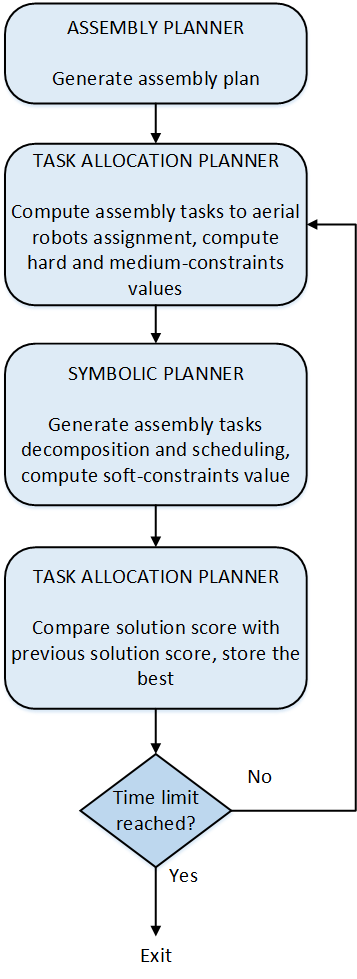
\includegraphics[width=0.40\columnwidth]{planning_algorithm.png}
    \caption[Planning algorithm.]{Work flow of the whole process where the role of the different planners is highlighted. }
    \label{fig:planning_algorithm}
\end{figure}

%After an assembly plan is generated, the task allocation planner computes an assembly tasks to aerial robots assignment, along with the hard and medium-constraints values. After that, the symbolic planner receives the assignment and decomposes the assembly tasks into low-level subtasks for the aerial robots, computing also its scheduling as well as the soft-constraints value. Once the solution score, which is composed by the hard-medium-soft values, is computed, then it is compared with the score of the previous solution, and the best is stored discarding the other. If the time limit has not been reached, then the process is repeated again.

The task allocation domain presented in Sect.~\ref{sec:optaplanner_domain} has been designed to solve the assignment part of the problem. In that domain only the aerial robots and assembly tasks along with its dependencies are considered as entities, but the temporal aspects of the problem are not present. The values of the hard and medium constraints are computed within this domain. The hard-constraint value indicates if the weight of the assigned parts does not exceed the sum of the payloads of the assigned aerial robots. Once an assembly task is allocated, the medium-constraint value indicates how many of its dependencies (parts that should be already assembled) are also allocated to the same aerial robot.

The symbolic domain presented in Sect.~\ref{sec:jshop2_domain} is designed to compute the assembly tasks decomposition and scheduling of the problem. In this case, the temporal domain is considered and the soft-constraint value is computed as the total assembly time for the whole structure within this symbolic domain.

The whole score calculation needs both planners to be connected and to communicate in a bidirectional way. First, the task allocation planner must solve the assignment problem and compute the related hard and medium constraints values. After that, it sends the computed assignment to the symbolic planner, which solves the decomposition and scheduling problem and computes the soft-constraint value. Then this value is send back to the task allocation planner, closing the score calculation loop. With the total score of the whole solution, the task allocation planner can compare different solutions and optimize the search to try to find new assignments that lead to better scores and improved solutions. Hence, the optimization is done cooperatively between the task allocation planner and the symbolic planner, preserving each of them its own domain and solving a different part of the whole problem.

\section{Simulation Results}
	\label{sec:results}

Different simulations have been carried out in the environment shown in Fig.~\ref{fig:environment}, which is the 3D model of the indoor testbed used for the experiments of the ARCAS Project. The tests have been done on a machine with an Intel i7 CPU at 2 GHz and 8GB RAM. The goal of the simulations is to compare different solvers at the task allocation planner level. 

\begin{figure}
    \centering
    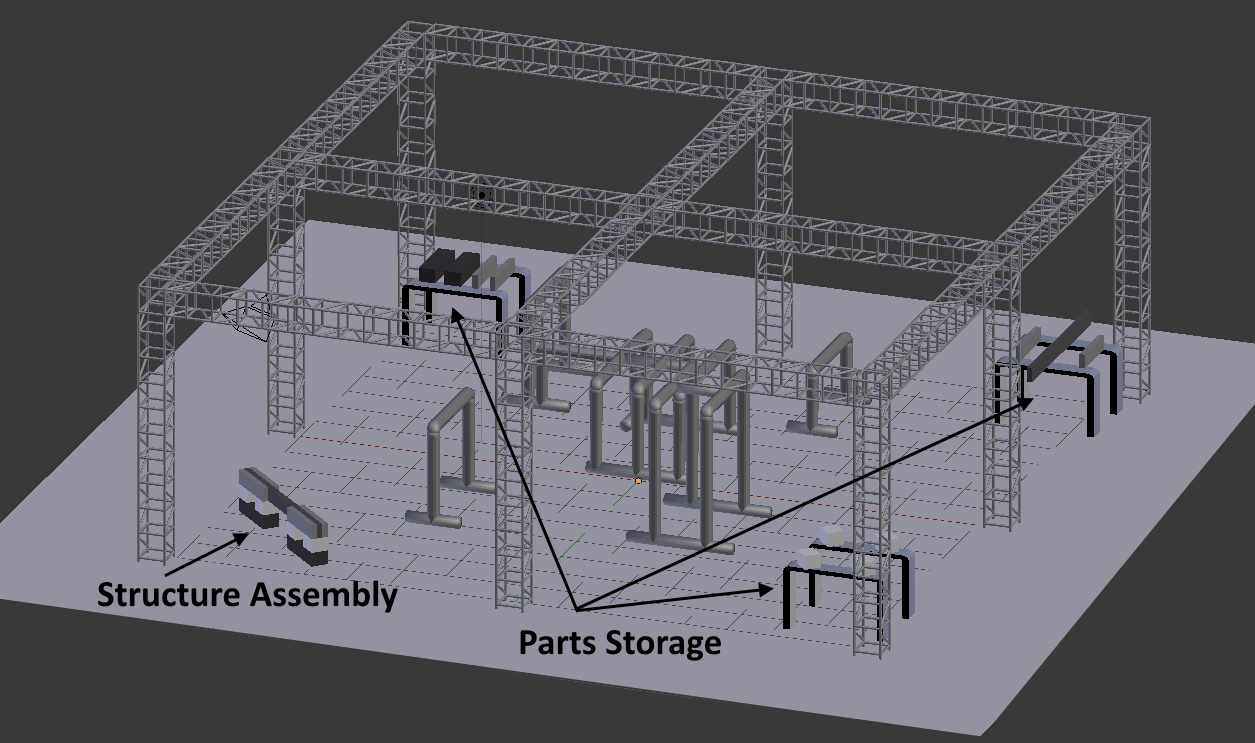
\includegraphics[width=0.99\columnwidth]{final_scene.png}
    \caption[Environment model of the mission.]{CAD model of the indoor testbed used for the experiments of the ARCAS Project. In this arena, the parts are initially stored over tables in different stock areas and are finally assembled on a designated location.}
    \label{fig:environment}
\end{figure}

A team of four aerial robots equipped with manipulators has to assemble a given structure. Three structures with different number of parts (Fig.~\ref{fig:structures}) have been considered and, for each of the structures, ten data sets have been generated changing randomly the initial locations of the parts. 

\begin{figure}
    \centering
    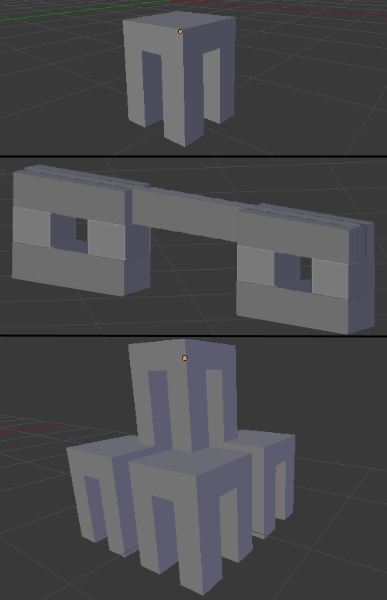
\includegraphics[width=0.45\columnwidth]{structures.png}
    \caption[Structures.]{Structures used for the benchmark with sizes of five, eleven and twenty-five parts (structures 1, 2 and 3 from top to bottom for later reference).}
    \label{fig:structures}
\end{figure}

The solver has been configured to use one Construction Heuristic phase followed by one Metaheuristic phase. The purpose of the former is to obtain an initial solution for the assignment problem, which will be later optimized by the second solver phase. Three CH algorithms have been applied to our problem: First Fit, First Fit Decreasing and Cheapest Insertion. A detailed description of each one can be found in~\cite{optaplanner_guide}. The results shown in Table~\ref{table:CH_score} have been computed with a time limit of ten minutes if the search does not finish before. It can be seen that the First Fit algorithm obtained better values, even reducing to zero the medium constraints. In addition, its computation times are lower than the others.

\begin{table}[htdp] 
		\caption{Construction Heuristic solver phase results for the 30 simulations. For each algorithm, the mean and standard deviations for the hard, medium and soft constraint values are presented, as well as the mean computation time. The broken constraints are represented as negative values. }
		\begin{tabular}{ | l | p{1cm} | p{1cm} | p{1cm} | c |}
	\hline
         CH Algorithm & Hard (SD) & Medium (SD) & Soft (SD) & Time(s)\\ \hline
         First Fit & -0.33 (0.48) & 0 (0) & -625.80 (418.34) & 3.12 \\ \hline
         First Fit Decreasing & -0.33 (0.48) & -0.33 (0.48) & -630.15 (422.36) & 9.56 \\ \hline
         Cheapest Insertion & -0.33 (0.48) & -0.33 (0.48) & -630.15 (422.36) & 21.33 \\ \hline
		\end{tabular}
	\label{table:CH_score}
\end{table}

The second phase is the MH phase, which tries to optimize the initial assignment computed by the previous CH phase. Five local search algorithms, whose description can also be found on~\cite{optaplanner_guide}, have been compared: Hill Climbing, Tabu Search, Simulated Annealing, Late Acceptance and Step Counting Hill Climbing. As this phase requires the use of a previous CH phase, the First Fit algorithm was configured as CH. The results are shown in Table~\ref{table:LS_score}. All the MH algorithms reduced to zero the values of the hard and medium constraints, so only the mean and standard deviations of the soft constraint values are shown. The results show that the Late Acceptance and Step Counting Hill Climbing algorithms tie, obtaining better values than the others.

\begin{table}
		\caption{Metaheuristics solver phase results generated after 30 simulations with three different structures. The solver was configured with a time limit of ten minutes if the search did not finish before. However, all the algorithms reached the time limit without exhausting the search. }
		\begin{tabular}{ | l | p{1cm} | p{1cm} | p{1cm} | p{1cm} |}
	\hline
         CH Algorithm & Structure 1 (SD) & Structure 2 (SD) & Structure 3 (SD) & Total (SD)\\ \hline
         Hill Climbing & -205.80 (14.19) & -415.80 (37.91) & -1020.0 (54.33) & -547.27 (353.15) \\ \hline
         Tabu Search & -205.80 (14.19) & -403.10 (29.64) & -1020.9 (55.95) & -543.27 (354.99) \\ \hline
         Simulated Annealing & -203.70 (15.29) & -413.40 (31.34) & -1031.9 (49.81) & -549.67 (359.18) \\ \hline
         Late Acceptance & -203.80 (15.33) & -410.80 (31.27) & -991.30 (73.75) & -535.30 (342.06) \\ \hline
         Step Counting H.C. & -203.80 (15.33) & -410.80 (31.27) & -991.30 (73.75) & -535.30 (342.06) \\ \hline         		\end{tabular}
	\label{table:LS_score}
\end{table}

Regarding scalability, one test with 50 robots and the structure of 25 parts was executed, configuring the Late Acceptance algorithm as metaheuristic along with the First Fit construction heuristic. The same setup was simulated with four robots and the results were compared. By increasing the number of robots, the number of solutions found was increased from 18 to 56 in ten minutes of simulation. This is due to the greater probability of finding an assignment that does not break any hard-constraint and thus leads to a feasible solution.

 %The new results obtained are compared with the originals on Table \ref{table:scalability_check}.
 
%\begin{table}
%\centering
%		\caption{In addition to the best score, the number of solutions obtained during the ten minutes time limit were compared. By increasing the number of aerial robots, the number of solutions found is increased. This is due of having a greater probability of finding an assignment of tasks to aerial robots that does not break any hard-constraint and thus leads to a feasible solution.}
%		\begin{tabular}{ | c | c | c |}
%		\hline
%         Aerial Robots & Best Score & Number of Solutions \\ \hline
%         4 & -846 & 18 \\ \hline
%         50 & -384 & 56 \\ \hline
%		 \hline
%         \end{tabular}
%	\label{table:scalability_check}
%\end{table}

Although it is out of the scope of this paper, our planning framework includes the possibility to simulate the execution of the low-level plans computed for each data set. An execution layer has been implemented as a C++ graphical user interface application to read the low-level plans. The interface, implemented using the Qt framework, checks for the correct execution and synchronization of the tasks and generates Gantt charts to display the different timelines of the aerial robots. The application communicates with a middleware developed by using the ROS (Robot Operating System) framework that connects with Gazebo simulator.

Figure~\ref{fig:sim2} shows a screenshot of a mission execution on the Gazebo simulator. A video of the execution, as well as the complete data sets used in this section, can be downloaded from \url{http://grvc.us.es/symballoc}.

\begin{figure}
    \centering
    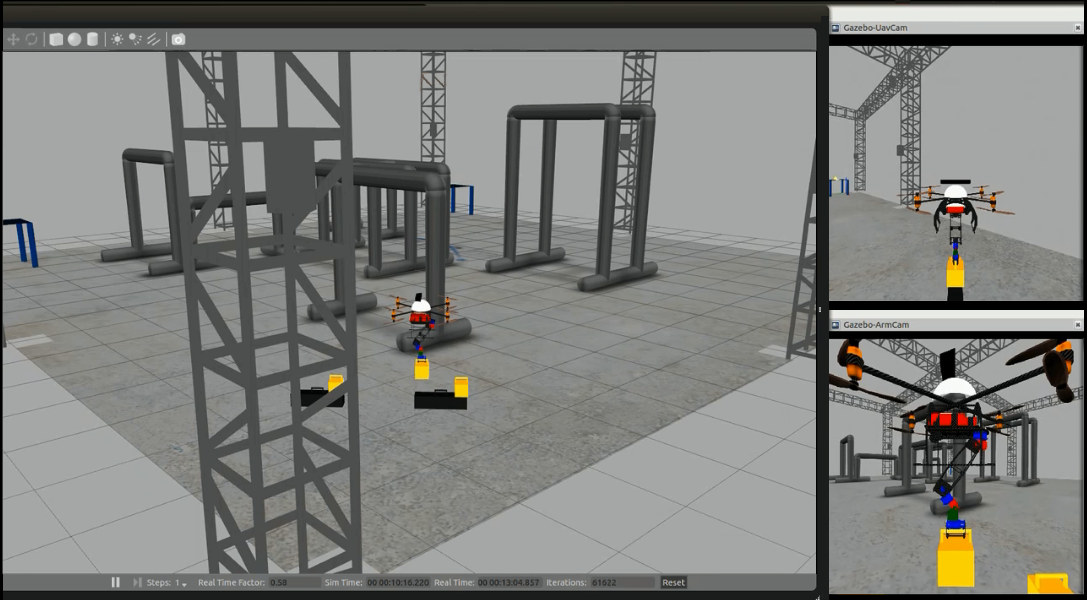
\includegraphics[width=0.99\columnwidth]{sim3.png}
    \caption[Simulation screenshot of an assembly action.]{Simulation screenshot of an assembly action executed by one aerial robot. All parts have a handle from which the aerial robots can take them and a cavity beneath that let them to be stacked.}
    \label{fig:sim2}
\end{figure}

\section{CONCLUSIONS AND FUTURE WORK}
	\label{sec:conclusions}

The planning engine presented performs task assignment and scheduling in order to increase the parallelism and cooperation in the mission. The main contribution of the paper is the successful connection of a task allocation planner with a symbolic planner in the context of structure assembly missions.

However, the approach has been tested in missions involving multiple simulated aerial robots. In future work, the goal is to execute the missions with the prototypes developed in the ARCAS Project in order to find more realistic aspects to enrich the planning domains. In addition, the symbolic planner domain designed needs to be optimized by reducing redundant preconditions present in the lower-level subtasks methods on which the high-level tasks are decomposed. Although redundant preconditions are a consequence of the inheritance among the high-level and lower-level task methods, they have an impact on computation times and can be deleted on lower-level methods if these are only used through the high-level tasks decomposition.

%\addtolength{\textheight}{-12cm}   % This command serves to balance the column lengths
                                  % on the last page of the document manually. It shortens
                                  % the textheight of the last page by a suitable amount.
                                  % This command does not take effect until the next page
                                  % so it should come on the page before the last. Make
                                  % sure that you do not shorten the textheight too much.

%-----------------------------------------------------------------------------
% BIBLIOGRAPHY
%-----------------------------------------------------------------------------
\bibliographystyle{IEEEtran}
\bibliography{IEEEabrv,bibliography}

\end{document}
